
%{{第五十二回}}{第五十二回}}

\chapter{俏平儿情掩虾须镯\hspace{.5em}勇晴雯病补雀金裘}

{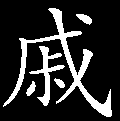
\includegraphics[width=3mm]{../Images/00005}  \kaishu 写黛玉弱症的是弱症,写晴雯时症的是时症;写湘云性快的是快性,写晴雯性傲的是傲性。彼何人斯?而具肖物手段如此。}

贾母道:``正是这话了。上次我要说这话,我见你们的大事多,如今又添出这些事来,你们固然不敢抱怨,未免想着我只顾疼这些小孙子孙女儿们,就不体贴你们这当家人了。你既这么说出来,更好了。''因此时薛姨妈李婶都在座,邢夫人及尤氏婆媳也都过来请安,还未过去,贾母向王夫人等说道:``今儿我才说这话,素日我不说,一则怕逞了凤丫头的脸,二则众人不伏。今日你们都在这里,都是经过妯娌姑嫂的,还有他这样想的到的没有?''薛姨妈、李婶、尤氏等齐笑说:``真个少有。别人不过是礼上面子情儿,实在他是真疼小叔子小姑子。就是老太太跟前,也是真孝顺。''贾母点头叹道:``我虽疼他,我又怕他太伶俐也不是好事。''凤姐儿忙笑道:``这话老祖宗说差了。世人都说太伶俐聪明,怕活不长。世人都说得,人人都信,独老祖宗不当说,不当信。老祖宗只有伶俐聪明过我十倍的,怎么如今这样福寿双全的?只怕我明儿还胜老祖宗一倍呢!我活一千岁后,等老祖宗归了西,我才死呢。''贾母笑道:``众人都死了,单剩下咱们两个老妖精,有什么意思。''说的众人都笑了。

宝玉因记挂着晴雯、袭人等事,便先回园里来。到房中,药香满屋,一人不见,只见晴雯独卧于炕上,脸面烧的飞红,又摸了一摸,只觉烫手。忙又向炉上将手烘暖,伸进被去摸了一摸身上,也是火烧。因说道:``别人去了也罢,麝月秋纹也这样无情,各自去了?''晴雯道:``秋纹是我撵了他去吃饭的,麝月是方才平儿来找他出去了。两人鬼鬼祟祟的,不知说什么。必是说我病了不出去。''宝玉道:``平儿不是那样人。况且他并不知你病特来瞧你,想来一定是找麝月来说话,偶然见你病了,随口说特瞧你的病,这也是人情乖觉取和的常事。便不出去,有不是,与他何干?你们素日又好,断不肯为这无干的事伤和气。''晴雯道:``这话也是,只是疑他为什么忽然间瞒起我来。''{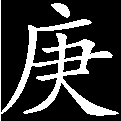
\includegraphics[width=3mm]{../Images/00004}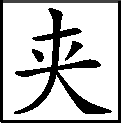
\includegraphics[width=3mm]{../Images/00012}\footnotesize \kaishu 宝玉一篇推情度理之谈以射正事,不知何如。}宝玉笑道:``让我从后门出去,到那窗根下听听说些什么,来告诉你。''说着,果然从后门出去,至窗下潜听。

只闻麝月悄问道:``你怎么就得了的?''{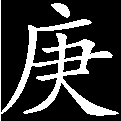
\includegraphics[width=3mm]{../Images/00004}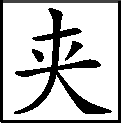
\includegraphics[width=3mm]{../Images/00012}\footnotesize \kaishu 妙!这才有神理,是平儿说过一半了。若此时从{(宝玉)}{[}平儿{]}口中从头说起一原一故,直是二人特等宝玉来听方说起也。}平儿道:``那日洗手时不见了,二奶奶就不许吵嚷,出了园子,即刻就传给园里各处的妈妈们小心查访。我们只疑惑邢姑娘的丫头,本来又穷,只怕小孩子家没见过,拿了起来也是有的。再不料定是你们这里的。幸而二奶奶没有在屋里,你们这里的宋妈妈去了,拿着这支镯子,说是小丫头子坠儿偷起来的,被他看见,来回二奶奶的。{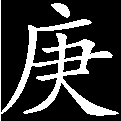
\includegraphics[width=3mm]{../Images/00004}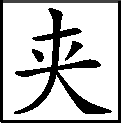
\includegraphics[width=3mm]{../Images/00012}\footnotesize \kaishu 妙极!红玉既有归结,坠儿岂可不表哉?可知``奸贼''二字是相连的。故``情''字原非正道,坠儿原不情也,不过一愚人耳,可以传奸即可以为盗。二次小窃皆出于宝玉房中,亦大有深意在焉。}我赶着忙接了镯子,想了一想:宝玉是偏在你们身上留心用意、争胜要强的,那一年有一个良儿偷玉,刚冷了一二年间,还有人提起来趁愿,这会子又跑出一个偷金子的来了。而且更偷到街坊家去了。偏是他这样,偏是他的人打嘴。所以我倒忙叮咛宋妈,千万别告诉宝玉,只当没有这事,别和一个人提起。第二件,老太太、太太听了也生气。三则袭人和你们也不好看。所以我回二奶奶,只说:`我往大奶奶那里去的,谁知镯子褪了口,丢在草根底下,雪深了没看见。今儿雪化尽了,黄澄澄的映着日头,还在那里呢,我就拣了起来。'二奶奶也就信了,所以我来告诉你们。你们以后防着他些,别使唤他到别处去。等袭人回来,你们商议着,变个法子打发出去就完了。''麝月道:``这小娼妇也见过些东西,怎么这么眼皮子浅。''平儿道:``究竟这镯子能多少重,原是二奶奶说的,这叫做`虾须镯',倒是这颗珠子还罢了。晴雯那蹄子是块爆炭,要告诉了他,他是忍不住的。一时气了,或打或骂,依旧嚷出来不好,所以单告诉你留心就是了。''说着便作辞而去。

宝玉听了,又喜又气又叹。喜的是平儿竟能体贴自己;气的是坠儿小窃;叹的是坠儿那样一个伶俐人,作出这丑事来。因而回至房中,把平儿之话一长一短告诉了晴雯。又说:``他说你是个要强的,如今病着,听了这话越发要添病,等好了再告诉你。''晴雯听了,果然气的蛾眉倒蹙,凤眼圆睁,即时就叫坠儿。宝玉忙劝道:``你这一喊出来,岂不辜负了平儿待你我之心了。不如领他这个情,过后打发他就完了。''晴雯道:``虽如此说,只是这口气如何忍得!''宝玉道:``这有什么气的?你只养病就是了。''

晴雯服了药,至晚间又服二和,夜间虽有些汗,还未见效,仍是发烧,头疼鼻塞声重。次日,王太医又来诊视,另加减汤剂。虽然稍减了烧,仍是头疼。宝玉便命麝月:``取鼻烟来,给他嗅些,痛打几个嚏喷,就通了关窍。''麝月果真去取了一个金镶双扣金星玻璃的一个扁盒来,递与宝玉。宝玉便揭翻盒扇,里面有西洋珐琅的黄发赤身女子,两肋又有肉翅,里面盛着些真正汪恰洋烟。{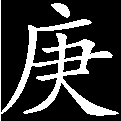
\includegraphics[width=3mm]{../Images/00004}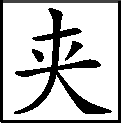
\includegraphics[width=3mm]{../Images/00012}\footnotesize \kaishu 汪恰,西洋一等宝烟也。}晴雯只顾看画儿,宝玉道:``嗅些,走了气就不好了。''晴雯听说,忙用指甲挑了些嗅入鼻中,不怎样。便又多多挑了些嗅入。忽觉鼻中一股酸辣透入囟门,接连打了五六个嚏喷,眼泪鼻涕登时齐流。{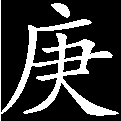
\includegraphics[width=3mm]{../Images/00004}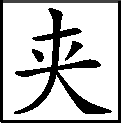
\includegraphics[width=3mm]{../Images/00012}\footnotesize \kaishu 写得出。}晴雯忙收了盒子,笑道:``了不得,好爽快!拿纸来。''早有小丫头子递过一搭子细纸,晴雯便一张一张的拿来醒鼻子。宝玉笑问:``如何?''晴雯笑道:``果觉通快些,只是太阳还疼。''宝玉笑道:``越性尽用西洋药治一治,只怕就好了。''说着,便命麝月:``和二奶奶要去,就说我说了:姐姐那里常有那西洋贴头疼的膏子药,叫做`依弗哪',找寻一点儿。''麝月答应了,去了半日,果拿了半节来。便去找了一块红缎子角儿,铰了两块指顶大的圆式,将那药烤和了,用簪挺摊上。晴雯自拿着一面靶镜,贴在两太阳上。麝月笑道:``病的蓬头鬼一样,如今贴了这个,倒俏皮了。二奶奶贴惯了,倒不大显。''说毕,又向宝玉道:``二奶奶说了:明日是舅老爷生日,太太说了叫你去呢。明儿穿什么衣裳?今儿晚上好打点齐备了,省得明儿早起费手。''宝玉道:``什么顺手就是什么罢了。一年闹生日也闹不清。''说着,便起身出房,往惜春房中去看画。

刚到院门外边,忽见宝琴的小丫鬟名小螺者从那边过去,宝玉忙赶上问:``那去?''小螺笑道:``我们二位姑娘都在林姑娘房里呢,我如今也往那里去。''宝玉听了,转步也便同他往潇湘馆来。不但宝钗姊妹在此,且连邢岫烟也在那里,四人围坐在熏笼上叙家常。紫鹃倒坐在暖阁里,临窗作针黹。一见他来,都笑说:``又来了一个!可没了你的坐处了。''宝玉笑道:``好一副`冬闺集艳图'!可惜我迟来了一步。横竖这屋子比各屋子暖,这椅子上坐着并不冷。''说着,便坐在黛玉常坐的搭着灰鼠椅搭一张椅上。因见暖阁之中有一玉石条盆,里面攒三聚五栽着一盆单瓣水仙,点着宣石,便极口赞:``好花!这屋子越发暖,这花香的越清香。昨日未见。''黛玉因说道:``这是你家的大总管赖大婶子送薛二姑娘的,两盆腊梅、两盆水仙。他送了我一盆水仙,他送了蕉丫头一盆腊梅。我原不要的,又恐辜负了他的心。你若要,我转送你如何?''宝玉道:``我屋里却有两盆,只是不及这个。琴妹妹送你的,如何又转送人,这个断使不得。''黛玉道:``我一日药吊子不离火,我竟是药培着呢,那里还搁的住花香来熏?越发弱了。况且这屋子里一股药香,反把这花香搅坏了。不如你抬了去,这花也清净了,没杂味来搅他。''宝玉笑道:``我屋里今儿也有病人煎药呢,你怎么知道的?''黛玉笑道:``这话奇了,我原是无心的话,谁知你屋里的事?你不早来听说古记,这会子来了,自惊自怪的。''

宝玉笑道:``咱们明儿下一社又有了题目了,就咏水仙腊梅。''黛玉听了,笑道:``罢,罢!我再不敢作诗了,作一回,罚一回,没的怪羞的。''说着,便两手握起脸来。宝玉笑道:``何苦来!又奚落我作什么。我还不怕臊呢,你倒握起脸来了。''宝钗因笑道:``下次我邀一社,四个诗题,四个词题。每人四首诗,四阕词。头一个诗题《咏〈太极图〉》,限一先的韵,五言律,要把一先的韵都用尽了,一个不许剩。''宝琴笑道:``这一说,可知是姐姐不是真心起社了,这分明难人。若论起来,也强扭的出来,不过颠来倒去弄些《易经》上的话生填,究竟有何趣味。我八岁时节,跟我父亲到西海沿子上买洋货,谁知有个真真国的女孩子,才十五岁,那脸面就和那西洋画上的美人一样,也披着黄头发,打着联垂,满头带的都是珊瑚、猫儿眼、祖母绿这些宝石;身上穿着金丝织的锁子甲洋锦袄袖;带着倭刀,也是镶金嵌宝的,实在画儿上的也没他好看。有人说他通中国的诗书,会讲五经,能作诗填词,因此我父亲央烦了一位通事官,烦他写了一张字,就写的是他作的诗。''众人都称奇道异。宝玉忙笑道:``好妹妹,你拿出来我瞧瞧。''宝琴笑道:``在南京收着呢,此时那里去取来?''宝玉听了,大失所望,便说:``没福得见这世面。''黛玉笑拉宝琴道:``你别哄我们。我知道你这一来,你的这些东西未必放在家里,自然都是要带了来的,这会子又扯谎说没带来。他们虽信,我是不信的。''宝琴便红了脸,低头微笑不语。宝钗笑道:``偏这个颦儿惯说这些白话,把你就伶俐的。''黛玉道:``若带了来,就给我们见识见识也罢了。''宝钗笑道:``箱子笼子一大堆还没理清,知道在那个里头呢!等过日收拾清了,找出来大家再看就是了。''又向宝琴道:``你若记得,何不念念我们听听?''宝琴方答道:``记得是首五言律,外国的女子也就难为他了。''宝钗道:``你且别念,等把云儿叫了来,也叫他听听。''说着,便叫小螺来吩咐道:``你到我那里去,就说我们这里有一个外国美人来了,作的好诗,请你这`诗疯子'来瞧去,再把我们`诗呆子'也带来。''小螺笑着去了。

半日,只听湘云笑问:``那一个外国美人来了?''一头说,一头果和香菱来了。众人笑道:``人未见形,先已闻声。''宝琴等忙让坐,遂把方才的话重叙了一遍。湘云笑道:``快念来听听。''宝琴因念道:

昨夜朱楼梦,今宵水国吟。

岛云蒸大海,岚气接丛林。

月本无今古,情缘自浅深。

汉南春历历,焉得不关心。

众人听了,都道:``难为他!竟比我们中国人还强。''一语未了,只见麝月走来说:``太太打发人来告诉二爷,明儿一早往舅舅那里去,就说太太身上不大好,不得亲自来。''宝玉忙站起来答应道:``是。''因问宝钗宝琴可去。宝钗道:``我们不去。昨儿单送了礼去了。''大家说了一回方散。

宝玉因让诸姊妹先行,自己落后。黛玉便又叫住他问道:``袭人到底多早晚回来。''宝玉道:``自然等送了殡才来呢。''黛玉还有话说,又不曾出口,出了一回神,便说道:``你去罢。''宝玉也觉心里有许多话,只是口里不知要说什么,想了一想,也笑道:``明日再说罢。''一面下了阶矶,低头正欲迈步,复又忙回身问道:``如今的夜越发长了,你一夜咳嗽几遍?醒几次?''{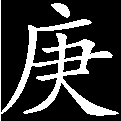
\includegraphics[width=3mm]{../Images/00004}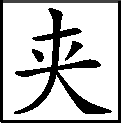
\includegraphics[width=3mm]{../Images/00012}\footnotesize \kaishu 此皆好笑之极,无味扯淡之极,回思则皆沥血滴髓之至情至神也。岂别部偷寒送暖,私奔暗约,一味淫情浪态之小说可比哉?}黛玉道:``昨儿夜里好了,只嗽两遍,却只睡了四更一个更次,就再不能睡了。''宝玉又笑道:``正是有句要紧的话,这会子才想起来。''一面说,一面便挨过身来,悄悄道:``我想宝姐姐送你的燕窝------''一语未了,只见赵姨娘走了进来瞧黛玉,问:``姑娘这两天好?''黛玉便知他是从探春处来,从门前过,顺路的人情。黛玉忙陪笑让坐,说:``难得姨娘想着,怪冷的,亲自走来。''又忙命倒茶,一面又使眼色与宝玉。宝玉会意,便走了出来。

正值吃晚饭时,见了王夫人,王夫人又嘱咐他早去。宝玉回来,看晴雯吃了药。此夕宝玉便不命晴雯挪出暖阁来,自己便在晴雯外边。又命将熏笼抬至暖阁前,麝月便在熏笼上。一宿无话。

至次日,天未明时,晴雯便叫醒麝月道:``你也该醒了,只是睡不够!你出去叫人给他预备茶水,我叫醒他就是了。''麝月忙披衣起来道:``咱们叫起他来,穿好衣裳,抬过这火箱\href{../Text/part0056_split_000.html\#lnkback_1_a}{\textsuperscript{①}}去,再叫他们进来。老嬷嬷们已经说过,不叫他在这屋里,怕过了病气。如今他们见咱们挤在一处,又该唠叨了。''晴雯道:``我也是这么说呢。''二人才叫时,宝玉已醒了,忙起身披衣。麝月先叫进小丫头子来,收拾妥当了,才命秋纹檀云等进来,一同伏侍宝玉梳洗毕。麝月道:``天又阴阴的,只怕有雪,穿那一套毡的罢。''宝玉点头,即时换了衣裳。小丫头便用小茶盘捧了一盖碗建莲红枣儿汤来,宝玉喝了两口。麝月又捧过一小碟法制紫姜来,宝玉噙了一块。又嘱咐了晴雯一回,便往贾母处来。

贾母犹未起来,知道宝玉出门,便开了房门,命宝玉进去。宝玉见贾母身后宝琴面向里也睡未醒。贾母见宝玉身上穿着荔色哆啰呢的天马箭袖,大红猩猩毡盘金彩绣石青妆缎沿边的排穗褂子。贾母道:``下雪呢么?''宝玉道:``天阴着,还没下呢!''贾母便命鸳鸯来:``把昨儿那一件乌云豹的氅衣给他罢。''鸳鸯答应了,走去果取了一件来。宝玉看时,金翠辉煌,碧彩闪灼,又不似宝琴所披之凫靥裘。只听贾母笑道:``这叫作`雀金呢',这是哦啰斯国拿孔雀毛拈了线织的。前儿把那一件野鸭子的给了你小妹妹,{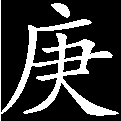
\includegraphics[width=3mm]{../Images/00004}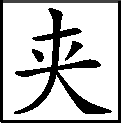
\includegraphics[width=3mm]{../Images/00012}\footnotesize \kaishu ``小''字更妙!盖王夫人之末女也。}这件给你罢。''宝玉磕了一个头,便披在身上。贾母笑道:``你先给你娘瞧瞧去再去。''宝玉答应了,便出来,只见鸳鸯站在地下揉眼睛。因自那日鸳鸯发誓决绝之后,他总不和宝玉讲话。宝玉正自日夜不安,此时见他又要回避,宝玉便上来笑道:``好姐姐,你瞧瞧,我穿着这个好不好。''鸳鸯一摔手,便进贾母房中来了。宝玉只得到了王夫人房中,与王夫人看了,然后又回至园中,与晴雯麝月看过后,至贾母房中回说:``太太看了,只说可惜了的,叫我仔细穿,别遭踏了他。''贾母道:``就剩下了这一件,你遭踏了也再没了。这会子特给你做这个也是没有的事。''说着又嘱咐他:``不许多吃酒,早些回来。''宝玉应了几个``是''。

老嬷嬷跟至厅上,只见宝玉的奶兄李贵和王荣、张若锦、赵亦华、钱启、周瑞六个人,带着茗烟、伴鹤、锄药、扫红四个小厮,背着衣包,抱着坐褥,笼着一匹雕鞍彩辔的白马,早已伺候多时了。老嬷嬷又吩咐了他六人些话,六个人忙答应了几个``是'',忙捧鞭坠镫。宝玉慢慢的上了马,李贵和王荣笼着嚼环,钱启周瑞二人在前引导,张若锦、赵亦华在两边紧贴宝玉后身。宝玉在马上笑道:``周哥,钱哥,咱们打这角门走罢,省得到了老爷的书房门口又下来。''周瑞侧身笑道:``老爷不在家,书房天天锁着的,爷可以不用下来罢了。''宝玉笑道:``虽锁着,也要下来的。''钱启李贵等都笑道:``爷说的是。便托懒不下来,倘或遇见赖大爷林二爷,虽不好说爷,也劝两句。有的不是,都派在我们身上,又说我们不教爷礼了。''周瑞钱启便一直出角门来。

正说话时,顶头果见赖大进来。宝玉忙笼住马,意欲下来。赖大忙上来抱住腿。宝玉便在镫上站起来,笑携他的手,说了几句话。接着又见一个小厮带着二三十个拿扫帚簸箕的人进来,见了宝玉,都顺墙垂手立住,独那为首的小厮打千儿,请了一个安。宝玉不识名姓,只微笑点了点头儿。马已过去,{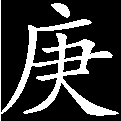
\includegraphics[width=3mm]{../Images/00004}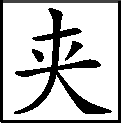
\includegraphics[width=3mm]{../Images/00012}\footnotesize \kaishu 总为后文伏线。}那人方带人去了。于是出了角门,门外又有李贵等六人的小厮并几个马夫,早预备下十来匹马专候。一出了角门,李贵等都各上了马,前引傍围的一阵烟去了,不在话下。

这里晴雯吃了药,仍不见病退,急的乱骂大夫,说:``只会骗人的钱,一剂好药也不给人吃。''{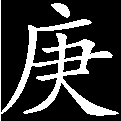
\includegraphics[width=3mm]{../Images/00004}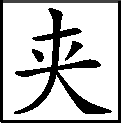
\includegraphics[width=3mm]{../Images/00012}\footnotesize \kaishu 奇文。真娇憨女儿之语也。}麝月笑劝他道:``你太性急了,俗语说:`病来如山倒,病去如抽丝。'又不是老君的仙丹,那有这样灵药!你只静养几天,自然好了。你越急越着手。''晴雯又骂小丫头子们:``那里钻沙去了!瞅我病了,都大胆子走了。明儿我好了,一个一个的才揭你们的皮呢!''唬的小丫头子篆儿忙进来问:``姑娘作什么?''{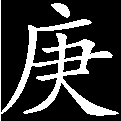
\includegraphics[width=3mm]{../Images/00004}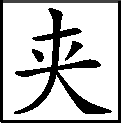
\includegraphics[width=3mm]{../Images/00012}\footnotesize \kaishu 此``姑娘''亦``姑姑''``娘娘''之称,亦如贾琏处小厮呼平儿,皆南北互用一语也。脂砚。}晴雯道:``别人都死绝了,就剩了你不成?''说着,只见坠儿也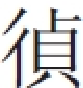
\includegraphics[width=4mm]{../images/00015}了进来。晴雯道:``你瞧瞧这小蹄子,不问他还不来呢。这里又放月钱了,又散果子了,你该跑在头里了。你往前些,我不是老虎吃了你!''坠儿只得前凑。晴雯便冷不防欠身一把将他的手抓住,{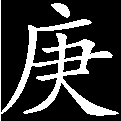
\includegraphics[width=3mm]{../Images/00004}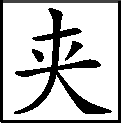
\includegraphics[width=3mm]{../Images/00012}\footnotesize \kaishu 是病卧之时。}向枕边取了一丈青,向他手上乱戳,口内骂道:``要这爪子作什么?拈不得针,拿不动线,只会偷嘴吃。眼皮子又浅,爪子又轻,打嘴现世的,不如戳烂了!''坠儿疼的乱哭乱喊。麝月忙拉开坠儿,按晴雯睡下,笑道:``才出了汗,又作死。等你好了,要打多少打不的?这会子闹什么!''晴雯便命人叫宋嬷嬷进来,说道:``宝二爷才告诉了我,叫我告诉你们,坠儿很懒,宝二爷当面使他,他拨嘴儿不动,连袭人使他,他背后骂他。今儿务必打发他出去,明儿宝二爷亲自回太太就是了。''宋嬷嬷听了,心下便知镯子事发,因笑道:``虽如此说,也等花姑娘回来知道了,再打发他。''晴雯道:``宝二爷今儿千叮咛万嘱咐的,什么`花姑娘'`草姑娘',我们自然有道理。你只依我的话,快叫他家的人来领他出去。''麝月道:``这也罢了。早也去,晚也去,带了去早清净一日。''

宋嬷嬷听了,只得出去唤了他母亲来,打点了他的东西,又来见晴雯等,说道:``姑娘们怎么了,你侄女儿不好,{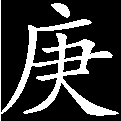
\includegraphics[width=3mm]{../Images/00004}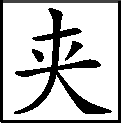
\includegraphics[width=3mm]{../Images/00012}\footnotesize \kaishu ``侄女''二字妙,余前注不谬。}你们教导他,怎么撵出去?也到底给我们留个脸儿。''晴雯道:``你这话只等宝玉来问他,与我们无干。''那媳妇冷笑道:``我有胆子问他去!他那一件事不是听姑娘们的调停?他纵依了,姑娘们不依,也未必中用。比如方才说话,虽是背地里,姑娘就直叫他的名字。在姑娘们就使得,在我们就成了野人了。''晴雯听说,一发急红了脸,说道:``我叫了他的名字了,你在老太太跟前告我去,说我撒野,也撵出我去。''麝月忙道:``嫂子,你只管带了人出去,有话再说。这个地方岂有你叫喊讲礼的?你见谁和我们讲过礼?别说嫂子你,就是赖奶奶林大娘,也得担待我们三分。便是叫名字,从小儿直到如今,都是老太太吩咐过的,你们也知道的,恐怕难养活,巴巴的写了他的小名儿,各处贴着叫万人叫去,为的是好养活。连挑水挑粪花子都叫得,何况我们!连昨儿林大娘叫了一声`爷',老太太还说他呢,此是一件。二则,我们这些人常回老太太的话去,可不叫着名字回话,难道也称`爷'?那一日不把宝玉两个字念二百遍,偏嫂子又来挑这个了!过一日嫂子闲了,在老太太、太太跟前,听听我们当着面儿叫他就知道了。嫂子原也不得在老太太、太太跟前当些体统差事,成年家只在三门外头混,怪不得不知我们里头的规矩。这里不是嫂子久站的,再一会,不用我们说话,就有人来问你了。有什么分证话,且带了他去,你回了林大娘,叫他来找二爷说话。家里上千的人,你也跑来,我也跑来,我们认人问姓,还认不清呢!''说着,便叫小丫头子:``拿了擦地的布来擦地!''那媳妇听了,无言可对,亦不敢久立,赌气带了坠儿就走。宋妈妈忙道:``怪道你这嫂子不知规矩,你女儿在这屋里一场,临去时,也给姑娘们磕个头。没有别的谢礼,------便有谢礼,他们也不希罕,------不过磕个头,尽了心。怎么说走就走?''坠儿听了,只得翻身进来,给他两个磕了两个头,又找秋纹等。他们也不睬他。那媳妇嗐声叹气,不敢多言,抱恨而去。

晴雯方才又闪了风,着了气,反觉更不好了,翻腾至掌灯,刚安静了些。只见宝玉回来,进门就嗐声跺脚。麝月忙问原故,宝玉道:``今儿老太太喜喜欢欢的给了这个褂子,谁知不防后襟子上烧了一块,幸而天晚了,老太太、太太都不理论。''一面说,一面脱下来。麝月瞧时,果见有指顶大的烧眼,说:``这必定是手炉里的火迸上了。这不值什么,赶着叫人悄悄的拿出去,叫个能干织补匠人织上就是了。''说着便用包袱包了,交与一个妈妈送出去。说:``赶天亮就有才好。千万别给老太太、太太知道。''婆子去了半日,仍旧拿回来,说:``不但能干织补匠人,就连裁缝绣匠并作女工的问了,都不认得这是什么,都不敢揽。''麝月道:``这怎么样呢!明儿不穿也罢了。''宝玉道:``明儿是正日子,老太太、太太说了,还叫穿这个去呢。偏头一日烧了,岂不扫兴。''

晴雯听了半日,忍不住翻身说道:``拿来我瞧瞧罢。没个福气穿就罢了,这会子又着急。''宝玉笑道:``这话倒说的是。''说着,便递与晴雯,又移过灯来,细看了一会。晴雯道:``这是孔雀金线织的,如今咱们也拿孔雀金线就像界线似的界密了,只怕还可混得过去。''麝月笑道:``孔雀线现成的,但这里除了你,还有谁会界线?''晴雯道:``说不得,我挣命罢了。''宝玉忙道:``这如何使得!才好了些,如何做得活。''晴雯道:``不用你蝎蝎螫螫的,我自知道。''一面说,一面坐起来,挽了一挽头发,披了衣裳,只觉头重身轻,满眼金星乱迸,实实撑不住。若不做,又怕宝玉着急,少不得恨命咬牙捱着。便命麝月只帮着拈线。晴雯先拿了一根比一比,笑道:``这虽不很像,若补上,也不很显。''宝玉道:``这就很好,那里又找哦啰嘶国的裁缝去。''{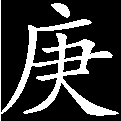
\includegraphics[width=3mm]{../Images/00004}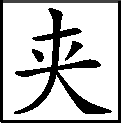
\includegraphics[width=3mm]{../Images/00012}\footnotesize \kaishu 妙谈!}晴雯先将里子拆开,用茶杯口大的一个竹弓钉牢在背面,再将破口四边用金刀刮的散松松的,然后用针纫了两条,分出经纬,亦如界线之法,先界出地子后,依本衣之纹来回织补。补两针,又看看,织补两针,又端详端详。无奈头晕眼黑,气喘神虚,补不上三五针,伏在枕上歇一会。宝玉在旁,一时又问:``吃些滚水不吃?''一时又命:``歇一歇。''一时又拿一件灰鼠斗篷替他披在背上,一时又命拿个拐枕与他靠着。急的晴雯央道:``小祖宗!你只管睡罢。再熬上半夜,明儿把眼睛抠搂了,怎么处!''宝玉见他着急,只得胡乱睡下,仍睡不着。一时只听自鸣钟已敲了四下,{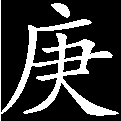
\includegraphics[width=3mm]{../Images/00004}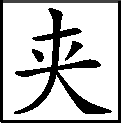
\includegraphics[width=3mm]{../Images/00012}\footnotesize \kaishu 按``四下''乃寅正初刻,``寅''此样写法,避讳也。}刚刚补完;又用小牙刷慢慢的剔出绒毛来。麝月道:``这就很好,若不留心,再看不出的。''宝玉忙要了瞧瞧,说道:``真真一样了。''晴雯已嗽了几阵,好容易补完了,说了一声:``补虽补了,到底不像,我也再不能了!''``嗳哟''了一声,便身不由主倒下。要知端的,且听下回分解。

{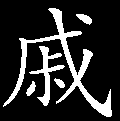
\includegraphics[width=3mm]{../Images/00005}  \kaishu 总评:此回前幅以药香、花香联络为章法,后幅以西洋鼻烟、西洋依弗哪药、西洋画儿、西洋诗、西洋哦}啰{嘶国雀金裘联络为章法,极穿插映带之妙。}

{写宝玉写不尽,却于仆从上描写一番。于管家见时描写一番,于园工诸人上描写一番。园中马是慢慢行,出门后又是一阵烟,大家气象、公子局度如画。}

{中一段写黛玉与宝玉满怀愁绪,有口难言,说不出一种凄凉,真是吴道子画顶上圆光。}

{\href{../Text/part0056_split_000.html\#navto_1_a}{①}原误``大箱'',据列、杨、甲辰本改,``火箱''即上文之``熏笼''。蒙、戚本此处作``熏笼'',下句``不叫他在这屋里''的``他''作``你'',似更合理。}
